\documentclass[11pt,libertine,widepage,nosubthm]{lmaths}
\addbibresource{../ors.bib}
\ExecuteBibliographyOptions{url=false}

\usepackage{tikz}
\usetikzlibrary{arrows}
\usetikzlibrary{cd}
\tikzcdset{arrow style=math font}

\newcommand{\ltlex}{<_{\mathrm{lex}}}
\newcommand{\gtlex}{>_{\mathrm{lex}}}
\setlist{leftmargin=3em}

\title{One-Relation Special Monoids Have Decidable Word Problems}
\author{}
\date{}

\let\oldbeginabstract\abstract
\renewcommand{\abstract}{\oldbeginabstract\noindent}

\newcommand{\draftnote}[1]{\textcolor{red}{#1}}
\newcommand{\nearrowstar}{\mathclap{\nearrow}_{\normalsize *}}
\newcommand{\searrowstar}{\mathclap{\searrow}^{\normalsize *}}

\begin{document}
\maketitle

\begin{abstract}%
This document is intended as a summary applying the techniques of \cite{Zhang1992a} to show that the word problem is decidable for monoids admitting a presentation of the form $\langle A \mid w = \epsilon\rangle$.
\end{abstract}


This note proves the following theorem, first proved by Adjan \cite{Adian1966}, using the approach of Zhang in \cite{Zhang1992a}:
\begin{theorem}[Adjan] \label{thm:ors-decidablewp}
	Let $M$ be a monoid admitting a presentation of the form $\langle A \mid u = \epsilon\rangle$, where $u$ is a word over a finite set $A$ of generators, and $\epsilon$ denotes (as it will henceforth) the empty word. Then the word problem of $M$ is decidable.
\end{theorem}

The broad approach is to use this presentation to derive a one-relation presentation for another monoid, which is shown to be a group to which we can reduce the word problem of the original monoid through a confluent, Noetherian rewriting system. We can then appeal to the corresponding word problem theorem for groups:
\begin{theorem}[Magnus] \label{thm:orgp-decidablewp}
	Let $G$ be a group admitting a presentation of the form $\langle A \mid u = v\rangle$, where $u$ and $v$ are words over the generating set $A$. Then the word problem for $G$ is decidable.
\end{theorem}

A proof of the above can be found in e.g. \cite{Magnus2004}.

Throughout, $\langle A \mid R \rangle$ will denote a monoid presentation; that is, the monoid obtained by taking the free monoid $A^*$ quotiented by the least congruence containing the elements $R \subseteq A^*$. We write $\Gp \langle A \mid R \rangle$ for group presentations, i.e. the quotients of free groups by the normal closures of a set of relators.


\section{Building a generating set}

Suppose $M = \langle A \mid w = \epsilon\rangle$ is a finitely presented monoid.

Given a subset $X \subseteq A^*$ of words, define
	\begin{align*}
		L(X) &= \{ x \in A^+ \mid \exists\ w \in A^* \colon wx \in X \} \text{ and } \\
		R(X) &= \{ x \in A^+ \mid \exists\ w \in A^* \colon xw \in X \}
	\end{align*}
to be the set of left and right factors respectively of words in $X$. Then, if $W(X) = L(X) \cap R(X)$ is the set of words which are both left and right factors, let $W'(X) = \{ w \in W(X) \mid \not\exists\ s, t \in A^+ \colon w = st, t \in W(X) \}$ be those two-sided factors for which no proper right factor appears in $W(X)$.

Taking $C_1 = \{w\}$, let
	\[ C_{i+1} = C_i \cup \{ xy \mid y \in W(C_i), yx \in C_i \} \cup \{ yz \mid y \in W(C_i), zy \in C_i \} \]
be those words obtained by moving right factors from $W(C_i)$ to the beginning of the words in $C_i$ in which they appear and left factors to the end of words. Each word in $C_i$ has the same length as $w$: this is easy to see by induction on $i$. It is clearly true in $C_1$. Suppose every word in $C_i$ has length $|w|$; then a new word $xy \in C_{i+1}$, with one of $x$ or $y \in W(C_i)$ has $xy$ or $yx$ in $C_i$ and hence $|xy| = |yx| = |w|$ by the inductive hypothesis. Hence every word in $C_{i+1}$ has length $|w|$.

It follows from this that since $|C_i| \le |A|^{|w|}$ (which is finite since $M$ is finitely presented) and $C_{i+1} \supseteq C_i$ for all $i \ge 1$, there is a maximal set $C_k$. The set $W'(C_k)$, denoted $E(M)$, shall form the generating set for the monoid we consider in the remainder of the proof.

\begin{example}
	We perform this construction on the monoid $M = \langle a, b \mid bbab = \epsilon \rangle$:

	\begin{center}
	\begin{tabular}{c|ll}
		$i$ & $C_i$ & $W(C_i)$ \\
		\hline
		1 & \{bbab\} & \{b, bbab\} \\
		2 & \{babb, bbab, bbba\} & \{bba, bb, b, bbab, bab, bbba, babb, ba\} \\
		3 & \{babb, bbab, abbb, bbba\} & \{ab, bba, abbb, bb, b, bbab, bab, bbb, bbba, a, babb, ba, abb\} \\
		4 & \{babb, bbab, abbb, bbba\} & \{ab, bba, abbb, bb, b, bbab, bab, bbb, bbba, a, babb, ba, abb\}
	\end{tabular}
	\end{center}

	The maximal set is $C_3 = \{babb, bbab, abbb, bbba\}$, so $E(M) = W'(C_3) = \{a, b\}$.
\end{example}

\begin{example}[The bicyclic monoid]
	Performing this construction on the bicyclic monoid $B = \langle b, c \mid bc = \epsilon \rangle$ gives the following:

	\begin{center}
	\begin{tabular}{c|ll}
		$i$ & $C_i$ & $W(C_i)$ \\
		\hline
		1 & \{bc\} & \{bc\} \\
		2 & \{bc\} & \{bc\}
	\end{tabular}
	\end{center}

	Hence the maximal set is $C_1 = \{bc\}$, giving $E(M) = W'(C_1) = \{ bc \}$.
\end{example}

\section{The group}
Define a new alphabet $B$ disjoint with $A$ such that we have a bijection $\midtilde\phi \colon E(M) \to B$, and let $\phi \colon E(M)^* \to B^*$ be the unique homomorphic extension of $\midtilde\phi$. By the following lemma, $\phi(w)$ is well-defined:

\begin{lemma} \label{lma:relator-factors-E(M)}
	The relator $w$ can be expressed as a product of factors in $E(M)$.
\end{lemma}
\begin{proof}
	\hspace{-0.25mm}We show that every element of $W(C_k)$ is a product of factors in $E(M)$. The lemma then follows since $w \in W(C_k)$.
	
	We proceed by induction on word length. Suppose $u \in W(C_k)$ is of minimal length in $W(C_k)$. Then $u$ has no proper factors in $W(C_k)$, and so $u \in E(M)$.

	Now suppose that all strings in $W(C_k)$ with length less than $n$ are products of factors in $E(M)$, and let $u \in W(C_k)$ have length $n$. If $u$ has no proper right factors in $W(C_k)$, then it is in $E(M)$ by definition. Otherwise, we can write $u = ev$ for $e \in E(M)$, $v \in A^+$. \draftnote{Why...?}

	Since $u$ is in $W(C_k)$, it is a prefix of some word $x \in C_k$, so that $x = ux' = e \cdot vx'$ for some $x' \in A^*$. The prefix $e$ is also in $W(C_k)$ --- since it is in $E(M)$ --- so by the definition of $C_{k+1}$, the word $vx'e$ is in $C_{k+1}$. But since $C_k$ is maximal, $C_{k+1} = C_k$, so $v$ is a prefix of a word in $C_k$.

	Furthermore, $u$ is also a suffix of some word in $C_k$, so $v$ is a suffix of the same word. Altogether, this means $v$ is in $W(C_k)$ and hence a product of factors in $E(M)$, by the inductive hypothesis. Therefore $u$ is a product of factors in $E(M)$, and by induction all the words of $W(C_k)$ can be expressed as such a product.
\end{proof}

We now define a monoid $M'$ given by the presentation $\langle B \mid \phi(w) = \epsilon \rangle$. We assert that this monoid is in fact a group:

\begin{lemma}
	The monoid $M' = \langle B \mid \phi(w) = \epsilon\rangle$ is a group.
\end{lemma}
\begin{proof}
	It suffices to show that every generator of $M'$ is invertible. We first show by induction that for all $i$, every word in $C_i$ is trivial in $M$. In the base case $C_1$, the only word to consider is $w$ itself, which is trivial by the defining relation $w = \epsilon$. Suppose then that all words in $C_j$ are trivial, for each $j \le i$, and consider a word $v \in C_{i+1}$, $v \not\in C_i$.

	In the first case, $v = xy$ for $y \in W(C_i)$, $yx \in C_i$. So by the inductive hypothesis, $yx =_M \epsilon$, i.e. $x$ is a right inverse for $y$ in $M$. As $y \in W(C_i)$, there is a word $u \in C_i$ such that $u = u'y =_M \epsilon$ for some $u' \in A^*$. So $u'$ is a left inverse for $y$ in $M$. We have a left and a right inverse for $y$ in $M$, so they must be equivalent in $M$, hence $v = xy =_M u'y =_M u$. But $u$ is in $C_i$ and so is trivial by the inductive hypothesis. Therefore $v =_M \epsilon$ as required.

	A similar argument shows that $v$ is trivial in $M$ if $v = yz$ for $y \in W(C_i)$, $zy \in C_i$. This accounts for every word in $C_{i+1}$, and so by induction all words in $C_j$ are trivial in $M$, for every index $j$. In particular, all the words in $C_k$ are trivial.

	For any word $z \in W(C_k)$, there are words $a, b$ in $C_k$ such that $a = za'$ and $b = b'z$ for some $a', b' \in A^*$. Since these words $a$ and $b$ are trivial in $M$, $a'$ is a right inverse for $z$ and $b'$ is a left inverse for $z$ in $M$ and hence $z$ is invertible in $M$. In particular, every word in $E(M)$ is invertible.

	Finally, if $b \in B$ is a generator of $M'$, then $\tilde\phi^{-1}(b) \in E(M)$ has an inverse $\midbar b$ in $M$. Then $\epsilon =_M \tilde\phi^{-1}(b) \midbar{b}$ and so $\epsilon =_{M'} b\phi(\midbar{b})$, and likewise $\phi(\midbar{b})b = \epsilon$. The arbitrary generator $b$ of $M'$ is hence invertible, so $M'$ is a group.
\end{proof}

We shall call this group $G$ rather than $M'$ from now on.

\pushcounter{example}{2}
\begin{example}
	Recall the monoid $M = \langle a, b \mid bbab = \epsilon \rangle$ from before. This presentation in fact presents a group; since $ba \leftrightarrow babbab \leftrightarrow bbabbabbab \leftrightarrow bbabab \leftrightarrow ab$, where $\leftrightarrow$ denotes the reflexive closure of the relation $\{(bbab, \epsilon)\}$, we have that $ba =_M ab$.
\end{example}
\popcounter{example}

\section{The rewriting system}
We use this group to construct a rewriting system on all the words of $A^*$, recalling that this is the set of all words over the generators of our original monoid.

A linear order on a set $X$ is a relation $<$ which is transitive and satisfies the trichotomy condition, i.e. exactly one of $x < y$ or $y < x$ or $x = y$ holds for all $x, y \in X$. Let $<$ be some linear order on the alphabet $A$, and extend it to a shortlex order $\ltlex$ over $A^*$: say that $x \ltlex y$ for words $x = x_1\cdots x_m$, $y = y_1\cdots y_n$ in $A^*$ if and only if $m < n$, or $m = n$ and there is some index $i$ such that $x_i < y_i$ and $x_j = y_j$ for all $1 \le j < i$.

Now define a rewriting system $R$ with precisely the rules $u \to v$, where $u, v \in E(M)^*$, $v \ltlex u$ and $\phi(u) =_G \phi(v)$.

This system $R$ is equivalent to the system $\{w \to \epsilon\}$, i.e. they present the same monoid:

\begin{lemma} \label{lma:R-equivalent-to-pres}
	The rewriting systems $\{w \to \epsilon\}$ and $R$ are equivalent in the sense that their Thue congruences are equal.
\end{lemma}
\begin{proof}
First, observe that $w \in E(M)^*$ by lemma \ref{lma:relator-factors-E(M)}, $\epsilon \ltlex w$, and $\phi(w) =_G \epsilon$ follows immediately from the presentation for $G$; so $w \to \epsilon$ is a rule in $R$ and hence $\leftrightarrow^*_{\{(w,\epsilon)\}}\ \subseteq\ \leftrightarrow^*_R$.

Conversely, suppose $u \to v$ is a rule in $R$. Then $\phi(u) =_G \phi(v)$ means $\phi(u) \leftrightarrow^*_{\{(\phi(w), \epsilon)\}} \phi(v)$, and since $\phi$ is a homomorphism, $u \leftrightarrow^*_{\{(w, \epsilon)\}} v$. So $\leftrightarrow^*_R\ \subseteq\ \leftrightarrow^*_{\{(w,\epsilon)\}}$.

Hence the two rewriting systems are equivalent.
\end{proof}

However, the advantage of $R$ over the simple system $\{w \to \epsilon\}$ is that it is confluent and Noetherian, and hence we can use it to find a unique normal form for every element in our one-relator monoid $M$. Once we have such a normal form, it is relatively straightforward to show \cref{thm:ors-decidablewp}, that the word problem is decidable.

\subsection{Some lemmas on $E(M)$}

We state here two lemmas about the generating set $E(M)$ which will be useful to prove the remaining properties of $R$:

\begin{lemma} \label{lma:no-middle-E(M)}
	If $x, y, z \in A^*$ are strings such that $xy, yz \in E(M)$, then either $y = \epsilon$ or $x = z = \epsilon$.
\end{lemma}
\begin{proof}
	Suppose $y \ne \epsilon$. Then since $xy \in E(M)$, $xy \in W(C_k)$ and in particular, $xy \in L(C_k)$, so there is some $\alpha \in A^*$ such that $\alpha x \cdot y \in C_k$. So $y$ is a right factor of a word in $C_k$, i.e. $y \in R(C_k)$. Likewise, $yz \in R(C_k)$ so $y \cdot z\beta \in C_k$ for some $\beta \in A^*$ and $y \in L(C_k)$. Hence $y \in W(C_k)$. By the definition of $E(M)$, $xy$ has no proper right factor in $W(C_k)$, so $y$ must not be a proper factor. By assumption, $y \ne \epsilon$, so we must have $x = \epsilon$. Similarly, $yz$ has no proper right factor in $W(C_k)$, so $z$ is not a proper factor and $z = \epsilon$.
\end{proof}

\begin{cly} \label{cly:middle-E(M)*}
	If $x, y, z \in A^*$ are strings such that $xy, yz \in E(M)^*$, then $y \in E(M)^*$.
\end{cly}
\begin{proof}
	Suppose $xy, yz \in E(M)^*$. Then we can factor
		\begin{align*}
			xy &= a_1 a_2 \cdots a_m, \\
			yz &= b_1 b_2 \cdots b_n
		\end{align*}
	for $a_i, b_i \in E(M)$. Then $y = X a_i a_{i+1} \cdots a_m$ for some index $i$ and some $X \in A^*$, and $y = b_1 \cdots b_j Z$ for some index $j, Y \in A^*$. \textcolor{red}{To be continued...}
\end{proof}


\subsection{Conditions for confluence}

In order to show that $R$ is a confluent rewriting system, we use the following condition for confluence, a restatement of theorem 1 in \cite{McNaughton1987}:
\begin{theorem}
	A rewriting system $R$ over an alphabet $A$ is confluent if and only if the following hold for all strings $u, v, w, x, y \in A^*$:
	\begin{enumerate}[(1)]
		\item \label{it:conf-overlap} If $uv \to x$ and $vw \to y$ are rules of $R$ then there is a $z \in A^*$ such that $xw \to^*_R z$ and $uy \to^*_R z$.
		\item \label{it:conf-middle} If $uvw \to x$ and $v \to y$ are rules of $R$ then there is a $z \in A^*$ such that $x \to^*_R z$ and $uyw \to^*_R z$.
	\end{enumerate}
\end{theorem}

Here, we shall prove this theorem for the restricted case of local confluence:

\begin{defn}
	A rewriting system $R$ over an alphabet $A$ is \dn{locally confluent} if for all strings $a, b, c \in A^*$, whenever $a \to_R b$ and $a \to_R c$, there exists a string $z \in A^*$ such that $b \to^*_R z$ and $c \to^*_R z$.
\end{defn}

This is sufficient for our purposes because $R$ is noetherian, and hence the following theorem applies:

\begin{theorem}[Newman] \label{thm:newman}
	If $R$ is a noetherian rewriting system, then $R$ is confluent if and only if it is locally confluent.
\end{theorem}

This theorem is often known as Newman's lemma, having first been proven by Newman in \cite{Newman1942}. A simpler proof written using the modern language of string rewriting systems appears in \cite{Huet1980}. The principal technique of this proof is the notion of \dn{Noetherian induction}:

\begin{prop}[Noetherian induction]
	Let $P(x)$ be a property of elements of a set $X$, and suppose that $\rightarrow$ is a noetherian relation. Then $P(x)$ is true for all $x$ if for any $y$, $P(y)$ is true if $P(z)$ is true for all $z \ne y$ such that $y \rightarrow^* z$.
\end{prop}
\begin{proof}
	Suppose $P(y)$ is true if $P(z)$ is true for all descendants $z$ of $y$, and suppose there is some $x \in X$ such that $P(x)$ is false. If $x$ has no descendants, then $P(x)$ is vacuously true. So $x$ must have a descendant $x_2$ such that $P(x_2)$ is false. By the same reasoning $x_2$ must have a descendant $x_3$ such that $P(x_3)$ is false. Continuing in this fashion, we have an infinite chain of descendants
		\[ \cdots \to x_3 \to x_2 \to x, \]
	for each of which $P$ is false. But this contradicts $\to$ being noetherian, since by definition a noetherian relation has no infinite chains.
\end{proof}

We can then proceed to the proof of theorem \ref{thm:newman}.

\begin{proof}[Theorem \ref{thm:newman}]
	Suppose $R$ is a locally confluent rewriting system over an alphabet $A$. We shall prove the statement $P(x)$ over $A^*$ by noetherian induction, where $P(x)$ is true if and only if for all $X, X' \in A^*$ such that $x \to^* X$ and $x \to^* X'$, there exists $z \in A^*$ such that $X \to^* z$ and $X' \to^* z$. By definition, if $P(x)$ holds for all strings, the system is confluent.

	Let $x \in A^*$ be such that $P(x)$ holds for all its descendants. Let $X, X' \in A^*$ be such that $x \to_R^* X$ and $x \to_R^* X'$, and in particular that $x = x_1 \to_R x_2 \to_R \cdots \to_R x_m = X$ and $x = x_1' \to_R x_2' \to_R \cdots \to_R x_n' = X'$. Since $R$ is locally confluent, the fact that $x \to_R x_1$ and $x \to_R x_1'$ means there exists a string $u \in A^*$ such that $x_1 \to_R^* u$ and $x_1' \to_R^* u$:

	{\centering
	\begin{tikzcd}
		& \arrow[dl] x \arrow[dr] \\
		x_1 \arrow[dd, "*"] \arrow[dr, "*"] & & x_1' \arrow[dd, "*"] \arrow[dl, "*"'] \\
		& u & \\
		X & & X'
	\end{tikzcd}
	\par}

	Since $x_1$ is a descendant of $x$, by the inductive hypothesis, there exists a $v \in A^*$ such that $u \to^* v$ and $X \to^* v$.

	{\centering
	\begin{tikzcd}
		& \arrow[dl] x \arrow[dr] \\
		x_1 \arrow[dd, "*"'] \arrow[dr, "*"] & & x_1' \arrow[dd, "*"] \arrow[dl, "*"'] \\
		& u \arrow[ddl, "*"] & \\
		X \arrow[d, "*"'] & & X' \\
		v
	\end{tikzcd}
	\par}

	Next, since $x_1'$ is a descendant of $x$, by the inductive hypothesis there is a string $w \in A^*$ such that $u \to^* w$ and $X' \to^* w$.

	{\centering
	\begin{tikzcd}
		& \arrow[dl] x \arrow[dr] \\
		x_1 \arrow[dd, "*"'] \arrow[dr, "*"] & & x_1' \arrow[dd, "*"] \arrow[dl, "*"'] \\
		& u \arrow[ddl, "*"] \arrow[ddr, "*"'] & \\
		X \arrow[d, "*"'] & & X' \arrow[d, "*"] \\
		v & & w
	\end{tikzcd}
	\par}

	To complete the proof, we observe that $u$ is a descendant of $x$, so there is a string $z \in A^*$ such that $v \to^* z$ and $w \to^* z$.

	{\centering
	\begin{tikzcd}
		& \arrow[dl] x \arrow[dr] \\
		x_1 \arrow[dd, "*"'] \arrow[dr, "*"] & & x_1' \arrow[dd, "*"] \arrow[dl, "*"'] \\
		& u \arrow[ddl, "*"] \arrow[ddr, "*"'] & \\
		X \arrow[d, "*"'] & & X' \arrow[d, "*"] \\
		v \arrow[dr, "*"] & & w \arrow[dl, "*"'] \\
		& z & 
	\end{tikzcd}
	\par}

	Thus we have found a $z$ such that $x_1 \to^* z$ and $x_1' \to^* z$ as required.
\end{proof}

With this in hand, we are now able to show the following:

\begin{theorem} \label{thm:local-confluence-cond}
	A noetherian rewriting system $R$ over an alphabet $A$ is confluent if and only if the following hold for all strings $u, v, w, x, y \in A^*$:
	\begin{enumerate}[(1)]
		\item \label{it:conf-overlap} If $uv \to x$ and $vw \to y$ are rules of $R$ then there is a $z \in A^*$ such that $xw \to^*_R z$ and $uy \to^*_R z$.
		\item \label{it:conf-middle} If $uvw \to x$ and $v \to y$ are rules of $R$ then there is a $z \in A^*$ such that $x \to^*_R z$ and $uyw \to^*_R z$.
	\end{enumerate}
\end{theorem}
\begin{proof}
	The `only if' direction is straightforward. To show the `if' direction, we prove $R$ is locally confluent; the result then follows from theorem \ref{thm:newman}.

	Suppose $a, x, y$ are strings such that $a \to_R x$ through a rule $u \to v$ and $a \to_R y$ through a rule $u' \to v'$. Then $a$ contains $u$ as a substring, i.e. $a = AuZ$ for some $A, Z \in A^*$. The string $u'$ must also occur somewhere in $a$. There are five possibilities for its location, and in each case we show that a common descendant $z \in A^*$ exists for $x$ and $y$ and hence that $R$ is locally confluent.

	\textbf{Case (i)}: $u'$ is entirely contained in $A$. Write $a = Bu'CuZ$, so that $A = Bu'C$. Then \[
		\begin{array}{lllll}
			& & Au'CvZ & & \\
			& \nearrow & & \searrow & \\
			a = Bu'CuZ & & & & Av'CvZ, \\
			& \searrow & & \nearrow & \\
			& & Av'CuZ & &
		\end{array}
	\]
	so $z = Av'CvZ$ works.

	\textbf{Case (ii)}: $u'$ is contained in $Au$ but not in $A$ or $u$. Factor $a = BCDEZ$ as follows, so that $u = DE$ and $u' = CD$:

	{\centering
	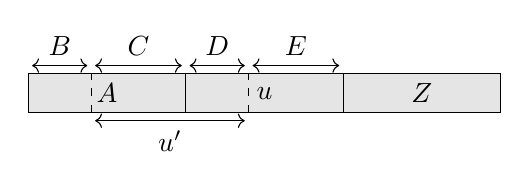
\begin{tikzpicture}
		\filldraw[fill=gray!20] (0,0) rectangle (2,0.5) node[midway] {$A$};
		\draw[<->] (0.05,0.6) -- (0.75,0.6) node[above,midway] {$B$};
		\draw[dashed] (0.8,0) -- (0.8,0.5);
		\draw[<->] (0.85,0.6) -- (1.95,0.6) node[above,midway] {$C$};
		\draw[solid] (2,0) -- (2,0.5);
		\filldraw[fill=gray!20] (2,0) rectangle (4,0.5) node[midway] {$u$};
		\draw[<->] (2.05,0.6) -- (2.75,0.6) node[above,midway] {$D$};
		\draw[<->] (0.85,-0.1) -- (2.75,-0.1) node [below,midway] {$u'$};
		\draw[dashed] (2.8,0) -- (2.8,0.5);
		\draw[<->] (2.85,0.6) -- (3.95,0.6) node[above,midway] {$E$};
		\filldraw[fill=gray!20] (4,0) rectangle (6,0.5) node[midway] {$Z$};
	\end{tikzpicture}\par}

	Then we have rules $CD \to v'$ and $DE \to v$ in $R$, so by hypothesis there is a $z \in A^*$ such that $v'E \to^*_R z$ and $Cv \to^*_R z$, and we have a common descendant like so: \[
		\begin{array}{lllll}
			& & Bv'EZ & & \\
			& \nearrow & & \searrowstar & \\
			a = BCDEZ & & & & BzZ. \\
			& \searrow & & \nearrowstar & \\
			& & BCvZ & &
		\end{array}
	\]

	\textbf{Case (iii)}: $u'$ is entirely contained in $u$. Factor $a = ABu'CZ$ so that $u = Bu'C$. Then by hypothesis there is a $z \in A^*$ such that $v \to^* z$ and $Bv'C \to^* z$. So we have the diagram: \[
		\begin{array}{lllll}
			& & ABv'CZ & & \\
			& \nearrow & & \searrowstar & \\
			a = ABu'CZ & & & & AzZ. \\
			& \searrow & & \nearrowstar & \\
			& & AvZ & &
		\end{array}
	\]

	\textbf{Case (iv)}: $u'$ is contained in $uZ$ but not in $u$ or $Z$. Factor $a = ABCDE$ as below, so that $u = BC$, $u' = CD$ and $Z = DE$:

	{\centering
	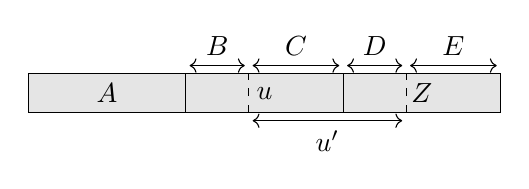
\begin{tikzpicture}
		\filldraw[fill=gray!20] (0,0) rectangle (2,0.5) node[midway] {$A$};
		\draw[<->] (2.05,0.6) -- (2.75,0.6) node[above,midway] {$B$};
		\draw[<->] (2.85,0.6) -- (3.95,0.6) node[above,midway] {$C$};
		\draw[solid] (2,0) -- (2,0.5);
		\filldraw[fill=gray!20] (2,0) rectangle (4,0.5) node[midway] {$u$};
		\draw[<->] (4.05,0.6) -- (4.75,0.6) node[above,midway] {$D$};
		\draw[dashed] (2.8,0) -- (2.8,0.5);
		\draw[<->] (4.85,0.6) -- (5.95,0.6) node[above,midway] {$E$};
		\filldraw[fill=gray!20] (4,0) rectangle (6,0.5) node[midway] {$Z$};
		\draw[dashed] (4.8,0) -- (4.8,0.5);
		\draw[<->] (2.85,-0.1) -- (4.75,-0.1) node [below,midway] {$u'$};
	\end{tikzpicture}\par}

	Since we have rules $BC \to v$, $CD \to v'$, by hypothesis there is a $z \in A^*$ such that $vD \to^* z$ and $Bv' \to z$, giving the diagram: \[
		\begin{array}{lllll}
			& & AvDE & & \\
			& \nearrow & & \searrowstar & \\
			a = ABCDE & & & & AzZ. \\
			& \searrow & & \nearrowstar & \\
			& & ABv'E & &
		\end{array}
	\]

	\textbf{Case (v)}: $u'$ is entirely contained in $Z$. This case is very similar to case (i) and is omitted.
\end{proof}

\subsection{Confluence of $R$}

We apply theorem \ref{thm:local-confluence-cond} from above directly to $R$ to show that it is confluent.

For part \ref{it:conf-overlap}, suppose $uv \to_R x$ and $vw \to_R y$, with $uv \ne vw$ (if they are equal, we have nothing to prove). We claim that in fact that one of $xw \to uy$ or $uy \to xw$ is a rule in $R$ and so $uy$ or $xw$ is a suitable $z$. By the definition of $R$, $uv, vw, x, y\in E(M)^*$, and so by \cref{cly:middle-E(M)*}, $v \in E(M)^*$. Hence $u, w \in E(M)^*$ and $uy, xw \in E(M)^*$. Now observe that by the rules we know are in $R$ and the fact $\phi$ is a homomorphism, we have $\phi(xw) = \phi(x)\phi(w) =_G \phi(uv)\phi(w) = \phi(u)\phi(vw) =_G \phi(u)\phi(y) = \phi(uy)$. Finally, since $\ltlex$ is linear, either $xw \ltlex uy$, in which case $uy \to xw$ is a rule in $R$; or $uy \ltlex xw$, in which case $xw \to uy$ is a rule in $R$ as required.

Now consider condition \ref{it:conf-middle}: suppose $uvw \to_R x$ and $v \to_R y$, and again assume that $v \ne y$. Observe that $\phi(x) =_G \phi(uyw)$, since $\phi(uvw) =_G \phi(x)$ and $\phi(v) =_G \phi(y)$. Furthermore, either $uyw \ltlex x$ or $x \ltlex uyw$. So as before, if $uyw \in E(M)^*$, then one of $x$ or $uyw$ will be a suitable $z$. Since $uvw, v, y \in E(M)^*$, if $uyw \not\in E(M)^*$, then $u = u_1u_2 \cdots u_m U$ and $w = W w_1 w_2 \cdots w_n$ for $u_i, w_i \in E(M)$ and some non-empty strings $U$ and $W$, with $UvW \in E(M)$. This means $v$ must be shorter than the longest word in $E(M)$ (or $UvW$ would be longer and therefore not in $E(M)$).

We claim that any word $a$ shorter than the longest word in $E(M)$ is irreducible under $R$: let $L$ be a word of maximal length in $E(M)$, and suppose $a$ were reducible. Then we can write $a = a'ba''$ where $b \in E(M)^*$ and $b \to_R c$ for some $c \in E(M)^*$. Then $c \ltlex b$ and so $|c| \le |b| \le |a| < |L|$, and hence $L$ cannot appear in $b$ or $c$. We then appeal to the Freiheitssatz for one-relator groups (found in \cite{Magnus2004}, although a more modern proof can be found in \cite{Lyndon2001}):

\begin{theorem}[Freiheitssatz]
	Let $G = \Gp \langle A \mid w = \epsilon \rangle$ be a one-relator group, and let $a \in A$ be a letter contained in $w$. Then the subgroup $\langle A \setminus \{a\} \rangle$ is a free group.
\end{theorem}

Since $b \to_R c$, $\phi(b) =_G \phi(c)$. Since $L$ is not in $b$ or $c$, $\phi(L)$ is not in $\phi(b)$ or $\phi(c)$, i.e. $\phi(b)$ and $\phi(c)$ are in the subgroup of $G$ generated by $B \setminus \{L\}$, which is free by the above; and so $\phi(b) = \phi(c)$ as words. Since $\phi$ is a homomorphism and $\midtilde\phi$ is a bijection, $\phi$ is injective and so $b = c$. But $c \ltlex b$, so we have a contradiction and $a$ is indeed irreducible.

It then follows that $v$ is irreducible by $R$; but this is impossible, since by hypothesis $v \to_R y$. So in fact $uyw \in E(M)^*$, and one of $uyw \to_R x$ or $x \to_R uyw$ holds. Therefore condition \ref{it:conf-middle} is satisfied and $R$ is confluent.


\subsection{Unique normal forms} \label{sec:unique-normal-forms}

That $R$ is Noetherian follows from the fact that $\ltlex$ is well-founded: pick a string $a$ and suppose there were an infinite chain of strings $a_1, a_2, \cdots \in A^*$ such that $a \gtlex a_1 \gtlex a_2 \gtlex \cdots$. All of these strings must be at most as long as $|a|$, and there are only finitely many (in fact, $|A|^{|a|}$) such strings. There is a string of length at most that of $|a|$ which is minimal with respect to $\gtlex$, namely the minimal letter $x$ in $A$ with respect to the linear order $<$ used to define $\ltlex$. Finally, since $\gtlex$ itself is linear, all of the $a_i$ must be distinct --- but this contradicts there being infinitely many of them.

Because $u \to^*_R v$ implies that $v \ltlex u$, this suffices to show that there is no infinite chain of strings $a_1 \to^*_R a_2 \to^*_R \cdots$, that is, that $R$ is Noetherian.

Since $R$ is Noetherian, given any word $w \in A^*$ representing a member of $M$, we can find an irreducible word $w'$ such that $w \leftrightarrow^*_{R} w'$, i.e. $w =_M w'$, by repeatedly applying rules from $R$. If we had another irreducible word $w''$ such that $w \leftrightarrow^*_{R} w''$, then because $R$ is confluent, there would be some $z$ such that $w' \to^*_R z$ and $w'' \to^*_R z$; but both $w'$ and $w''$ are irreducible, so in fact $z = w' = w''$. Hence each word $w$ has a \emph{unique} irreducible word in $A^*$, the normal form of $w$, denoted $\midbar{w}$.


\section{The word problem is decidable}

We now prove \cref{thm:ors-decidablewp}.

Let $v, w \in A^*$ be words representing members of $M$. By the argument in \cref{sec:unique-normal-forms}, both $v$ and $w$ have unique normal forms $\midbar{v}$ and $\midbar{w}$ with respect to the rewriting system $R$. To find the normal form for $v$, set $v_1 = v$. We find the string $v_{i+1}$ from $v_i$ by iterating over the rules in $R$ to determine which could apply to $v_i$. This can be done in finitely many steps since there are only finitely many strings in $E(M)^*$ which have length at most $|v_i|$ (and any longer strings could not occur in $v_i$). We can then iterate over every pair of such strings to decide whether $v \ltlex u$. Finally, since the word problem is decidable for one-relator groups (\cref{thm:orgp-decidablewp}), it is decidable in finite time whether $\phi(u) =_G \phi(v)$.

Once we have a set of candidate rewrite rules, apply any of them to $v_i$ to get $v_{i+1}$, or terminate with $\midbar{v} = v_i$ if there are none remaining. Since $R$ is Noetherian, the process will always terminate in this manner.

Using the same procedure to compute $\midbar{w}$, we can now determine whether $v$ and $w$ are equal in $M$: since $R$ is equivalent to $\{w \to \epsilon\}$, $v =_M w$ if and only if $v \leftrightarrow^*_R w$, which is the case if and only if $\midbar{v} = \midbar{w}$, we can determine whether $v =_M w$ or $v \ne_M w$ by comparing $\midbar v$ and $\midbar w$ letter by letter. This comparison completes in finitely many steps for arbitrary $v$ and $w$, as does the computation of $\midbar v$ and $\midbar w$, so the word problem for $M$ is decidable.

\printbibliography


\end{document}
